\documentclass[tikz,border=12pt]{standalone}
\usepackage{graphicx}
\usepackage{amsmath,amssymb}
\usepackage{tikz}
\usetikzlibrary{arrows.meta,positioning,fit,calc,backgrounds}
\tikzset{
  box/.style={
    draw,
    very thick,
    rectangle,
    align=center,
    inner sep=8pt,
    minimum height=1.25cm,
    minimum width=3.1cm,
    font=\small,
  },
  wide/.style={box, minimum width=3.6cm},
  arr/.style={-{Stealth[length=2.6mm, width=2mm]}, thick},
  barr/.style={
    {Stealth[length=2.4mm, width=1.8mm]}-{Stealth[length=2.4mm, width=1.8mm]},
    thick,
  },
  lbl/.style={font=\scriptsize, inner sep=2pt, fill=white},
  group/.style={draw, dashed, inner sep=12pt},
}

\begin{document}
\definecolor{gin}{RGB}{236,236,236}
\definecolor{gre}{RGB}{157,181,125}
\definecolor{red}{RGB}{233,120,128}
\definecolor{ora}{RGB}{238,175,100}
% stacked block: name, cx, cy, w, h, colour, label (rotated)
\newcommand{\stk}[7]{%
  \draw[rounded corners=4pt, draw=black!35, fill=#6!22] (#2-#4/2-0.42,#3-#5/2-0.42) rectangle (#2+#4/2-0.42,#3+#5/2-0.42);
  \draw[rounded corners=4pt, draw=black!45, fill=#6!48] (#2-#4/2-0.21,#3-#5/2-0.21) rectangle (#2+#4/2-0.21,#3+#5/2-0.21);
  \node[rounded corners=4pt, draw=black!70, thick, fill=#6, minimum width=#4 cm, minimum height=#5 cm, inner sep=1pt, font=\normalsize, align=center] (#1) at (#2,#3) {\rotatebox{90}{#7}};}
\tikzset{
  gbox/.style={rounded corners=4pt, draw=black!60, thick, fill=gin, align=center, font=\small, inner sep=8pt},
  panel/.style={draw=ora!85!black, dashed, thick, rounded corners=8pt, fill=ora!6},
  plbl/.style={font=\large\bfseries, text=black!70},
  a/.style={-{Stealth[length=3mm,width=2.2mm]}, very thick, draw=black!75},
  al/.style={font=\footnotesize, align=center, fill=white, inner sep=2pt},
}
\begin{tikzpicture}
  % ---------------- panels (all same height) ----------------
  \draw[panel] (-4.2,-9.6) rectangle (13.8,13.4);
  \draw[panel] (15.0,-9.6) rectangle (31.6,13.4);
  \draw[panel] (32.8,-9.6) rectangle (46.2,13.4);
  \node[plbl, anchor=north west] at (-4.0,13.2) {(a) Shared: identical for both agents};
  \node[plbl, anchor=north west] at (15.2,13.2) {(b) Internal model: the one difference};
  \node[plbl, anchor=north west] at (33.0,13.2) {(c) Outputs: same};

  % ---------------- (a) inputs + frozen encoder ----------------
  \node[gbox, minimum width=7.2cm] (cam) at (0,8.3) {%
    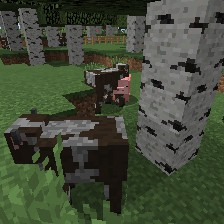
\includegraphics[width=4.8cm]{img/cam_frame.png}\\[4pt]
    \textbf{Camera frame}: what the agent sees\\$224\times224$ colour image};
  \stk{dino}{0}{1.8}{6.4}{2.6}{gre}{}
  \node[font=\large, align=center] at (0,1.8) {\textbf{DINOv2}\\frozen};
  \draw[a] (cam) -- (dino);
  \node[gbox, minimum width=7.2cm, fill=ora!22] (prop) at (0,-5.3) {%
    \textbf{Proprioception}: 11 numbers\\[3pt]
    \footnotesize
    \begin{tabular}{@{}l@{\hspace{8pt}}l@{}}
      on ground          & 0 (airborne)\\
      yaw / pitch        & 0.69 (125$^\circ$) / 0.30 (27$^\circ$)\\
      velocity (y, x, z) & 0, 0, 0\\
      position vs.\ spawn & $-1.2$, $1.0$, $8.8$\\
      food / health      & 1.0 / 1.0
    \end{tabular}};
  \node[font=\footnotesize\itshape, align=center] at (0,-8.7) {real example, same time step from a recorded episode};

  % observation vector: tall, narrow horizontal trapezoid, light colour coding
  \fill[gre!45]  (9.8,8.4) -- (12.6,4.4) -- (12.6,-1.0) -- (9.8,-3.9) -- cycle;
  \fill[ora!40]  (9.8,-3.9) -- (12.6,-1.0) -- (12.6,-2.6) -- (9.8,-7.2) -- cycle;
  \draw[very thick, draw=black!70, rounded corners=2pt] (9.8,8.4) -- (12.6,4.4) -- (12.6,-2.6) -- (9.8,-7.2) -- cycle;
  \draw[thick, draw=black!70] (9.8,-3.9) -- (12.6,-1.0);
  \node[font=\small, align=center] at (11.0,3.0) {\textbf{image}\\\textbf{features}};
  \node[font=\small, align=center] at (10.9,-4.2) {\textbf{proprio}};
  \node[font=\normalsize, align=center] at (11.2,10.4) {\textbf{Observation vector}\\\textbf{6,539} numbers};
  \node[font=\footnotesize\itshape, align=center] at (11.2,-8.4) {bands not\\drawn to scale};
  \draw[a] (dino.east) -- node[al, above=2pt] {17 tokens $\times$ 384\\= 6,528 numbers} (9.8,1.8);
  \draw[a] (prop.east) -- node[al, above=2pt] {11 numbers\\(skips DINOv2)} (9.8,-5.3);

  % ---------------- (b) the two internal models ----------------
  \stk{ppoin}{17.9}{5.6}{2.2}{5.8}{gre}{Input layers}
  \stk{ppom}{22.1}{5.6}{2.6}{5.8}{red}{Feedforward layer}
  \node[font=\normalsize, align=left, anchor=south west] at (24.3,5.95) {\textbf{PPO}\\no memory\\\textit{learns:}\\on-policy rollouts,\\GAE, clipped loss};
  \stk{drin}{17.9}{-5.6}{2.2}{5.8}{gre}{Input layers}
  \stk{drm}{22.1}{-5.6}{2.6}{5.8}{red}{RSSM world model}
  \node[font=\normalsize, align=left, anchor=south west] at (24.3,-5.25) {\textbf{Dreamer}\\recurrent memory\\\textit{learns:}\\fit model on replay,\\policy in imagination};
  \draw[a] (12.6,0.7) -- ++(1.2,0) |- (ppoin.west);
  \draw[a] (12.6,0.7) -- ++(1.2,0) |- (drin.west);
  \draw[a] (ppoin) -- (ppom);
  \draw[a] (drin) -- (drm);

  % ---------------- (c) heads and outputs ----------------
  \stk{act}{35.6}{5.0}{2.0}{5.0}{gre}{Actor head}
  \stk{crt}{35.6}{-5.0}{2.0}{5.0}{gre}{Critic head}
  \node[gbox, minimum width=5.0cm, minimum height=3.2cm] (oa) at (42.2,5.0) {\textbf{action}\\1 of 12: move, turn,\\jump, attack, \dots};
  \node[gbox, minimum width=5.0cm, minimum height=3.2cm] (ov) at (42.2,-5.0) {\textbf{value} $V$\\expected future reward};
  \draw[very thick, draw=black!75] (ppom.east) -- (31.9,5.6) -- (31.9,-5.6) -- (drm.east);
  \draw[a] (31.9,0) -- (33.4,0) |- (act.west);
  \draw[a] (33.4,0) |- (crt.west);
  \draw[a] (act) -- (oa);
  \draw[a] (crt) -- (ov);
  \node[font=\footnotesize\itshape, align=center] at (39.5,0) {same architecture\\in both agents};
\end{tikzpicture}
\end{document}
